\newpage

\section{Abstract}

\emph{Hamiltonian cycles} are a very interesting problem lining all
undergraduate discrete mathematics textbooks. At a higher level, we understand
them as complex to solve. Here we look at the problem and discuss intricate
details that have allowed the development of relatively efficient but still
exponential algorithms for solving Hamiltonian Cycles.

\section{Introduction}

The \emph{Hamiltonian Cycle Problem} is a problem that has been known for a very
long time to be hard. Hamiltonian Cycles are often used to study the fundamental
theories and understanding of complexity theory. Here we assume graphs are
undirected, the conversion from undirected to directed graphs is not difficult
however.

\subsection{Hamiltonian Paths and Hamiltonian Cycles Definition}

The hamiltonian cycle is similar to that of the hamiltonian path where inside an
undirected or directed graph, the hamiltonian path, also known as the traceable
path, is a path that visits each vertex exactly once. However, differing to the
hamiltonian path, the starting point and ending point of the path must also be
adjacent to each other such that they are able to create a cycle using an
available edge.

\begin{center}
    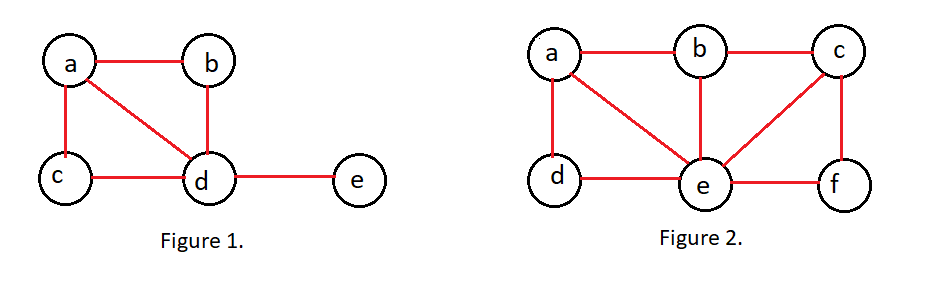
\includegraphics[width=\textwidth]{image2}
\end{center}

In figure 1, there are multiple paths inside the undirected graph that result in
a hamiltonian path, but due to the requirement of needing to start with node
$e$, there is no hamiltonian cycle since there is no edge that accomplishes the
requirement of the starting node and ending node of the path to connect.

Figure 2 shows an example of an undirected graph that includes a hamiltonian
cycle as, starting with any node, such as $a$, allows for a path such as
$abcfeda$ or $adefcba$, fulfilling the criteria of connecting the first and last
nodes.

\subsection{Mathematical Definition}

\begin{definition}[Graph]
    A graph $G$ is a tuple with a set of verticies $V$ and edges $E$, with an
    edge connecting two verticies. Notated as $G = (V, E)$
\end{definition}

\begin{definition}[Path for Undirected Graphs \cite{Ros0701}]
    Let $n$ be a nonnegative integer and $G$ an undirected graph. A path of
    length $n$ from $u$ to $v$ in $G$ is a sequence of $n$ edges $e_1,...,e_n$
    of $G$ for which there exists a sequence of $x_0 = u$, $x_1, ..., x_{n-1}$,
    $x_n = v$ of vertices such that $e_i$ has for $i = 1, ..., n$, the endpoints
    $x_{i-1}$ and $x_i$.
\end{definition}

\begin{definition}[A Cycle \cite{Ros0701}]
    A graph has a cycle if it has a path where $u = v$.
\end{definition}

\begin{definition}[A Simple Cycle or Path \cite{Ros0701}]
    A path or cycle is simple if all its edges appear in the path only once.
\end{definition}


\begin{definition}[Hamiltonian Cycle \cite{Ros0702}]
    A Hamiltonian Cycle is a simple cycle that visits all the vertices in a
    graph.
\end{definition}

\begin{definition}[Forced Edge \cite{Epps2007}]
    A edge is forced if it must appear in the Hamiltonian Cycle.
\end{definition}

\subsection{The Hamiltonian Cycle Problem}

There are many variations of the Hamiltonian Cycle Problem.

The decision problem Hamilton Cycle Problem would be to find if a hamiltonian
cycle exists or not. The decision problem can be extended to what is generally
understood as the hamiltonian path problem by returning the path if it exists.
The decision problem is NP-complete. Another variation of the Hamiltonian Cycle
Problem is to find how many hamiltonian cycles exist in a graph.

Not all graphs have equivalent complexity. Some graphs are relatively trivial to
solve in exact exponential time with very small, near polynomial bases. This
property makes Hamiltonian Cycles an interesting problem to research when
looking at a search space for algorithms that solve the hamiltonian cycle
problem. Unrelated to our implementations in this report, it has been
hypothesised that the hardest graphs to solve lie close to the bound
$\frac{1}{2} v \cdot \ln(v)+\frac{1}{2} \ln(\ln(v))$ \cite{Szem2006}. It also
has been shown through empirical methods \cite{Berg2021} that there exists
graphs that are difficult to solve far away from this bound. 

The \emph{Travelling Salesman Problem} is reducible to the Hamiltonian Cycle
Problem by setting the weight of the graph to 1. As a direct result, many of the
algorithms used to solve the hamiltonian cycle problem were originally intended
as a solution to the travelling salesman problem.

\subsection{Overview and Restrictions}

Hamiltonian Cycles have been known for a long time to be solvable through a
brute-force depth-first search. At the same time, this yields less efficient
time complexity. Bellman\cite{Bell1962}, Held and Karp\cite{Karp1962} developed
a dynamic programming algorithm for solving travelling salesman in exact
exponential time that applies to the Hamiltonian Cycle Problem. It was shown
after that not all graphs have equal complexity, and by restricting a graph to
degree 3 \cite{Epps2007}, there exists an exact exponential bound with a near
polynomial base, as long as the graph was restricted to having at most vertices
with degree 3.

\newpage

\section{Algorithms}

\subsection{Backtracking 1: Brute Force DFS}

The backtracking algorithm is a brute-force approach to problem solving and
involves “backtracking” if the current solution is not suitable. That is, the
algorithm attempts to recursively build a solution, one step at a time, and if
the resulting solution fails, another solution will be found by trying another
solution and/or moving one step back, eventually finding every single solution
to the problem.

In regards to the hamiltonian cycle problem:

\textbf{Step 0:}

We first create an adjacency matrix to the undirected graph to make finding the
hamiltonian cycle easier. This involves writing ‘1’ where there is a connection
between the next vertex, and ‘0’ where there is none.

\begin{figure}[h]
    \centering
    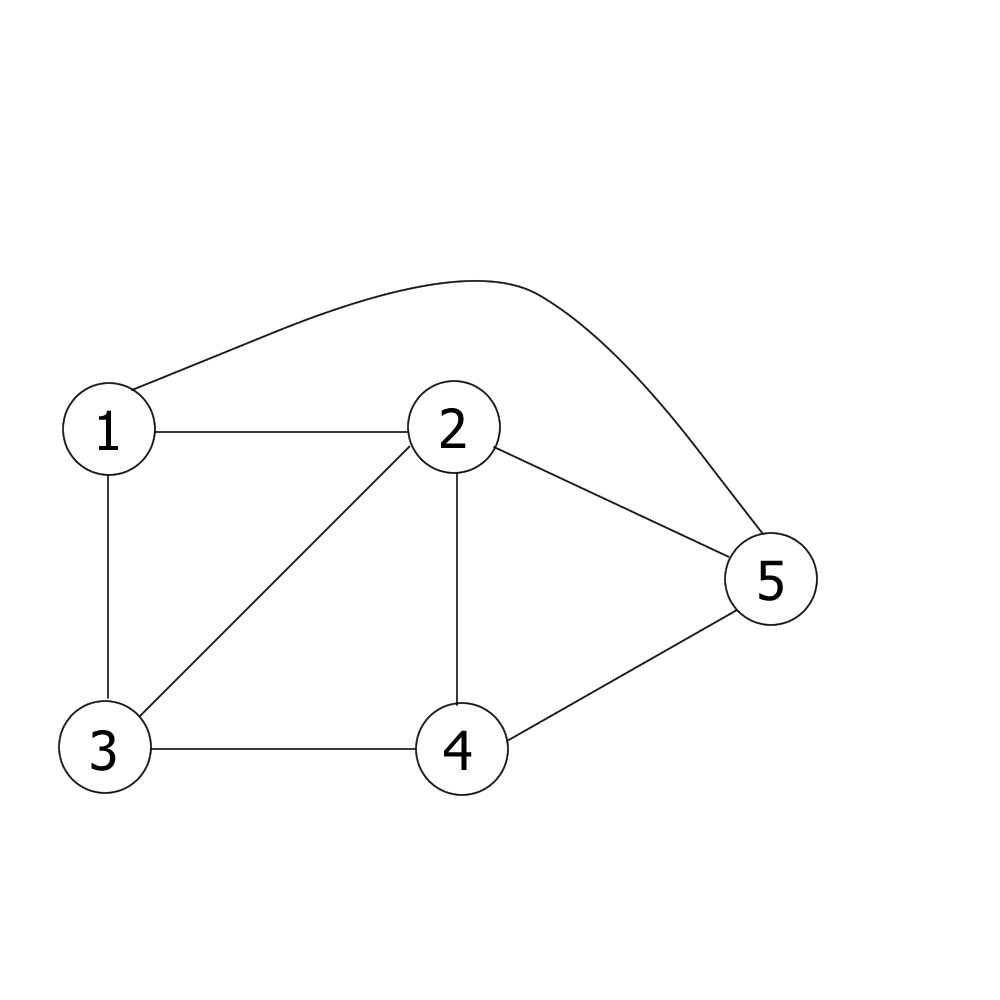
\includegraphics[width=8cm]{image3}
    \caption{Example Graph 1. Undirected Graph}
    \label{fig:a}
\end{figure}

\begin{table}[h]
    \centering
    \caption{Example Adjacency Matrix}
    \begin{tabular}{l | lllll}
          & 0 & 1 & 2 & 3 & 4  \\
        \hline
        0 & 0 & 1 & 1 & 0 & 1  \\
        1 & 1 & 0 & 1 & 1 & 1  \\
        2 & 1 & 1 & 0 & 1 & 0  \\
        3 & 0 & 1 & 1 & 0 & 1  \\
        4 & 1 & 1 & 0 & 1 & 0 
    \end{tabular}
\end{table}

\textbf{Step 1:}

We will first create an empty array to store the hamiltonian path.

\begin{table}[H]
    \centering
    \caption{Path Array}
    \begin{tabular}{l | lllll}
        index & 0 & 1 & 2 & 3 & 4  \\
        \hline
        value &   &   &   &   &    \\
    \end{tabular}
\end{table}

\textbf{Step 2:}

We will then fill in the first node in the graph.

\begin{table}[H]
    \centering
    \caption{Path Array}
    \begin{tabular}{l | lllll}
        index & 0 & 1 & 2 & 3 & 4  \\
        \hline
        value & 1 &   &   &   &    \\
    \end{tabular}
\end{table}

This will result in the following path.

\begin{figure}[H]
    \centering
    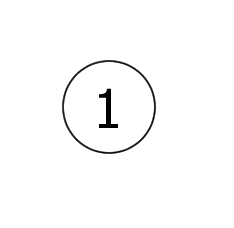
\includegraphics[width=4cm]{image18}
\end{figure}

\textbf{Step 3:}

We will then attempt to increment the next node into the array.

\begin{table}[H]
    \centering
    \caption{Path Array}
    \begin{tabular}{l | lllll}
        index & 0 & 1 & 2 & 3 & 4  \\
        \hline
        value & 1 & {\cellcolor[rgb]{0.933,0.804,0.804}}1 &   &   &    \\
    \end{tabular}
\end{table}

However, since 1 is already in the path, the value will be incremented again.

\begin{table}[H]
    \centering
    \caption{Path Array}
    \begin{tabular}{l | lllll}
        index & 0 & 1 & 2 & 3 & 4  \\
        \hline
        value & 1 & 2 &   &   &    \\
    \end{tabular}
\end{table}

This new value will then be compared against the adjacency matrix to check if
the previous node (node 1) is adjacent to the current node (node 2).

\begin{table}[H]
    \centering
    \begin{tabular}{l | lllll}
          & 0 & 1 & 2 & 3 & 4  \\
        \hline
        0 & 0 & {\cellcolor[rgb]{0.863,0.914,0.835}}1 & 1 & 0 & 1  \\
        1 & 1 & 0 & 1 & 1 & 1  \\
        2 & 1 & 1 & 0 & 1 & 0  \\
        3 & 0 & 1 & 1 & 0 & 1  \\
        4 & 1 & 1 & 0 & 1 & 0 
    \end{tabular}
\end{table}

As there is a ‘1’ in the adjacency matrix when matching node 1 with node 2, this
means that the path is valid, making the following path:

\begin{figure}[H]
    \centering
    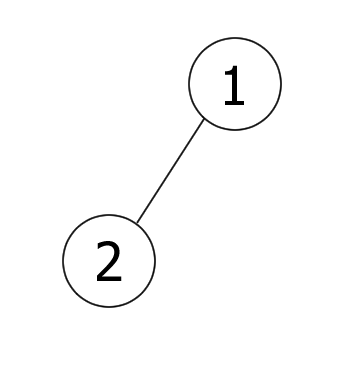
\includegraphics[width=4cm]{image11}
\end{figure}

\textbf{Step 4:}

To show this again, the same steps will be repeated with index 3.
We will then attempt to increment the next node into the array.

\begin{table}[H]
    \centering
    \caption{Path Array}
    \begin{tabular}{l | lllll}
        index & 0 & 1 & 2 & 3 & 4  \\
        \hline
        value & 1 & 2 & {\cellcolor[rgb]{0.933,0.804,0.804}}1 &   &    \\
    \end{tabular}
\end{table}

However, since 1 is already in the path, the value will be incremented again.

\begin{table}[H]
    \centering
    \caption{Path Array}
    \begin{tabular}{l | lllll}
        index & 0 & 1 & 2 & 3 & 4  \\
        \hline
        value & 1 & 2 & {\cellcolor[rgb]{0.933,0.804,0.804}}2 &   &    \\
    \end{tabular}
\end{table}

However, since 2 is already in the path, the value will be incremented again.

\begin{table}[H]
    \centering
    \caption{Path Array}
    \begin{tabular}{l | lllll}
        index & 0 & 1 & 2 & 3 & 4  \\
        \hline
        value & 1 & 2 & 3 &   &    \\
    \end{tabular}
\end{table}

This new value will then be compared against the adjacency matrix to check if
the previous node (node 2) is adjacent to the current node (node 3).

\begin{table}[H]
    \centering
    \begin{tabular}{l | lllll}
          & 0 & 1 & 2 & 3 & 4  \\
        \hline
        0 & 0 & 1 & 1 & 0 & 1  \\
        1 & 1 & 0 & 1 & 1 & 1  \\
        2 & 1 & {\cellcolor[rgb]{0.863,0.914,0.835}}1 & 0 & 1 & 0  \\
        3 & 0 & 1 & 1 & 0 & 1  \\
        4 & 1 & 1 & 0 & 1 & 0 
    \end{tabular}
\end{table}

As there is a ‘1’ in the adjacency matrix when matching node 2 with node 3, this
means that the path is valid, making the following graph:

\begin{figure}[H]
    \centering
    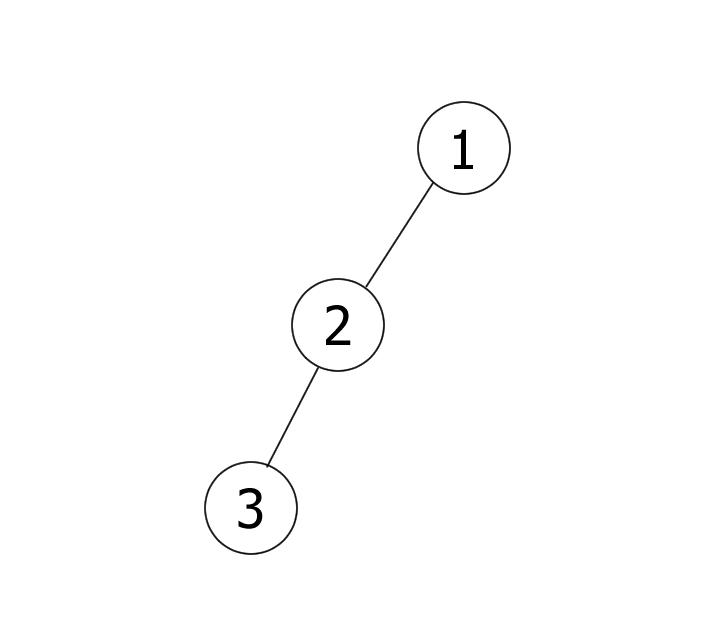
\includegraphics{image17}
\end{figure}

This will be continued until it fills in the entire array. An issue that can
occur is if the new node is invalid, in which it will just increment and test
the next node. For example, given the following graph and adjacency matrix:

\textbf{Invalid Adjacency}

\begin{figure}[H]
    \centering
    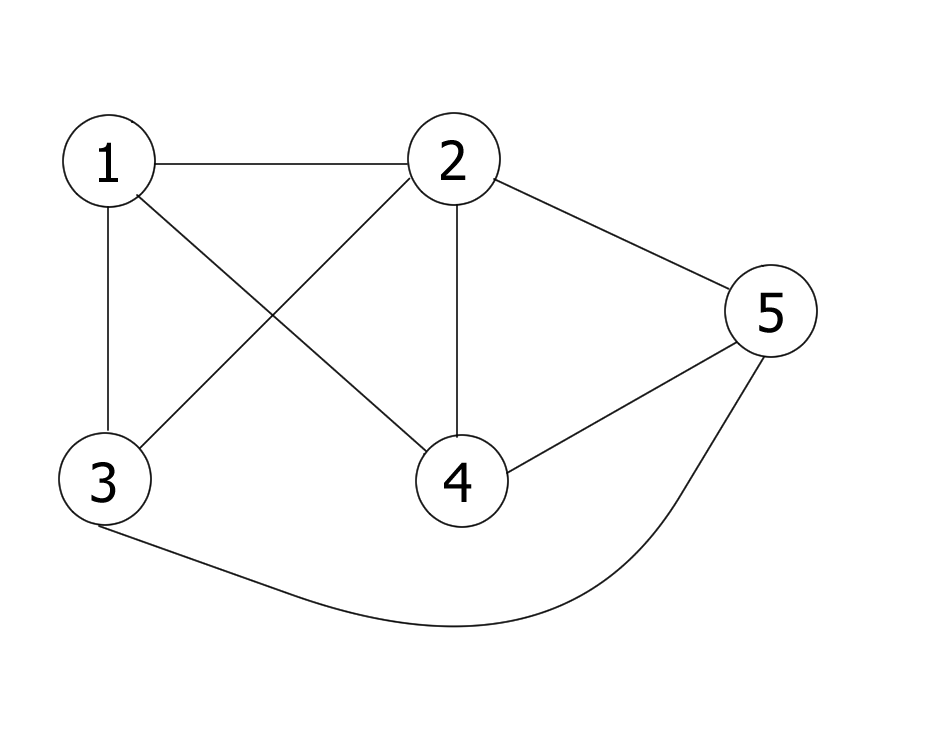
\includegraphics{image8}
    \caption{Example Graph 2: Invalid Adjacency}
\end{figure}

\begin{table}[H]
    \centering
    \begin{tabular}{l | lllll}
          & 0 & 1 & 2 & 3 & 4  \\
        \hline
        0 & 0 & 1 & 1 & 0 & 1  \\
        1 & 1 & 0 & 1 & 1 & 1  \\
        2 & 1 & 1 & 0 & 1 & 0  \\
        3 & 0 & 1 & 1 & {\cellcolor[rgb]{0.933,0.804,0.804}}0 & 1  \\
        4 & 1 & 1 & 0 & 1 & 0 
    \end{tabular}
\end{table}


\begin{table}[H]
    \centering
    \caption{Path Array}
    \begin{tabular}{l | lllll}
        index & 0 & 1 & 2 & 3 & 4  \\
        \hline
        value & 1 & 2 & 3 & {\cellcolor[rgb]{0.933,0.804,0.804}}4 &  \\
    \end{tabular}
\end{table}

As 4 is not a valid adjacent node, it will try incrementing again.

\subsection{Backtracking 2: Eppsteins Algorithm}

By considering possible permutations of a graph with degree 3. Eppstein was able
to develop an algorithm that had the time-complexity $O(2^{\frac{3n}{8}})$ and
in linear space \cite{Epps2007}. The algorithm was a careful backtracking
technique that identified all possible permutations of a cubic graph and defined
a set of back tracking rules.

\subsection{Dynamic Programming: Held-Karps Algorithm}

